\chapter{Implementation of Proposed G-FLCS for Radial Plasma Position Control in Aditya Tokamak Fusion Test Reactor}
\begin{chapterAbstract}{Preview}
	In this chapter, a nonlinear process plant, Aditya Tokamak Fusion Test Reactor (TFTR) is controlled by the proposed G-FLCS. Tokamak is a torus shaped magnetic field based confinement device for the extremely hot plasma. It is one of the most widely researched device since it is key to only form of clean energy that can be industrially generated. To stabilize the plasma across radial position is crucial to the success of a tokamak reactor. Plasma is highly sensitive and nonlinear state of a matter and its position control is extremely time critical. In this chapter, the proposed hardware based G-FLCS controller is used to control Radial Plasma Position in Aditya TFTR, installed at Institute of Plasma Research (IPR), Gandhinagar, India.
\end{chapterAbstract}
\clearpage

\section{Introduction}
In last chapter, a remotely tunable MT-FRHC based G-FLCS with VBCoA is implemented on TI C6748 DSP. A HIL test was also conducted to see the performance of this system. In this chapter, the proposed G-FLCS is used to control the radial position of a plasma column in Aditya Tokamak Fusion Test Reactor (TFTR). Aditya TFTR is installed at installed at Institute of Plasma Research (IPR), Gandhinagar, India. It is a medium size tokamak with major radius of 0.75 m and a minor radius of 0.25 m. There are 20 toroidal field coils in the design which produces a maximum field strength of 1.2 tesla. Genetic algorithm based FCP is used to extract FCP which can drive the G-FLCS in controlling the radial plasma position in the torus. The FCP can also be extracted partly using conventional optimization methods. Gradient Descent, Back propagation and other stochastic methods are employed to derive the co-ordinates of the antecedent membership functions \cite{Nguyen1996,Nguyen2003,Nguyen2015}. When the rules are defined the conventional optimization methods may be used provided the cost function is convex in nature. However, mostly it is not true. Moreover, the output of the FLC is not a continuous function. So optimizing the antecedents and consequents are not possible at same instance. Thus, evolutionary algorithms are preferred, specially Genetic Algorithm, owing to its ease of implementation has been used in this work \cite{Bandyopadhyay2001a,Surmann2001,Jajulwar200919}.
 
\subsection{Controlled Thermonuclear Fusion}
Researchers observed that there was an enormous release of energy that occurred when two light nuclei (with masses lower than iron, Fe, in periodic table) fuse together. This phenomenon was termed as thermonuclear fission reaction. Then, World War II ended with an historical uncontrolled thermonuclear fusion, the bombings at Hiroshima and Nagasaki. At this time, many scientist and engineers realized that if this phenomenon can be confined and controlled, the possibility of harnessing this energy for development of mankind would be enormous. A thermonuclear fusion can be confined and controlled by
\begin{itemize}
	\item Gravitational confinement
	\item Magnetic confinement
	\item Inertial confinement
	\item Electrostatic confinement 
\end{itemize}

\subsection{Tokamak Fusion Reactor}
A tokamak is a magnetic field based plasma confining device in the shape of a torus. A stable plasma equilibrium can be achieved by generating magnetic field lines which can helically  move around the torus. The plasma position control in a Tokamak reactor is a highly nonlinear control problem. In Tokamak reactor, magnetic field is used to confine the plasma in desired position. Plasma is highly sensitive state of matter and can be unstable under slightest trigger in the surrounding environment. It is therefore very important to design a fast but highly robust controller. A tokamak can successfully operate if the plasma is stable and confined to the geometric center of the vacuum vessel. The radial position of the confined plasma inside the torus vessel inflict on the quality of the plasma discharge. Unstable plasma when approaches too close to the wall of the vessel, it may lead to partial or complete disruption of the plasma. Hence it is of primal importance that the plasma position is controlled throughout the plasma discharge process.

To achieve a stable plasma equilibrium and to confine it inside, a fusion reactor is required to generate magnetic field lines that helically embraces the torus shaped plasma. These magnetic field lines can be generated using electromagnets positioned accordingly. Generation of helical field can be achieved by adding a magnetic field that circularly travels around the torus (toroidal field) and another field that travels orthogonally across to the toroidal field (poloidal field). These field are generated by toroidal field coils and inner and outer poloidal field coils as shown in Figure \ref{fig:Tokamak}. When a current is passed to a centrally located helical inner poloidal magnetic field coil, it produces an induced current in the plasma. Direction of the coil current and induced plasma current is shown in red arrows. This plasma current generates a poloidal magnetic field. The required toroidal magnetic field is produced by the circularly surrounded coils across the torus. The position of the plasma can be controlled by driving the electric current to these coils. 
\begin{figure}[h!]
	\centering
	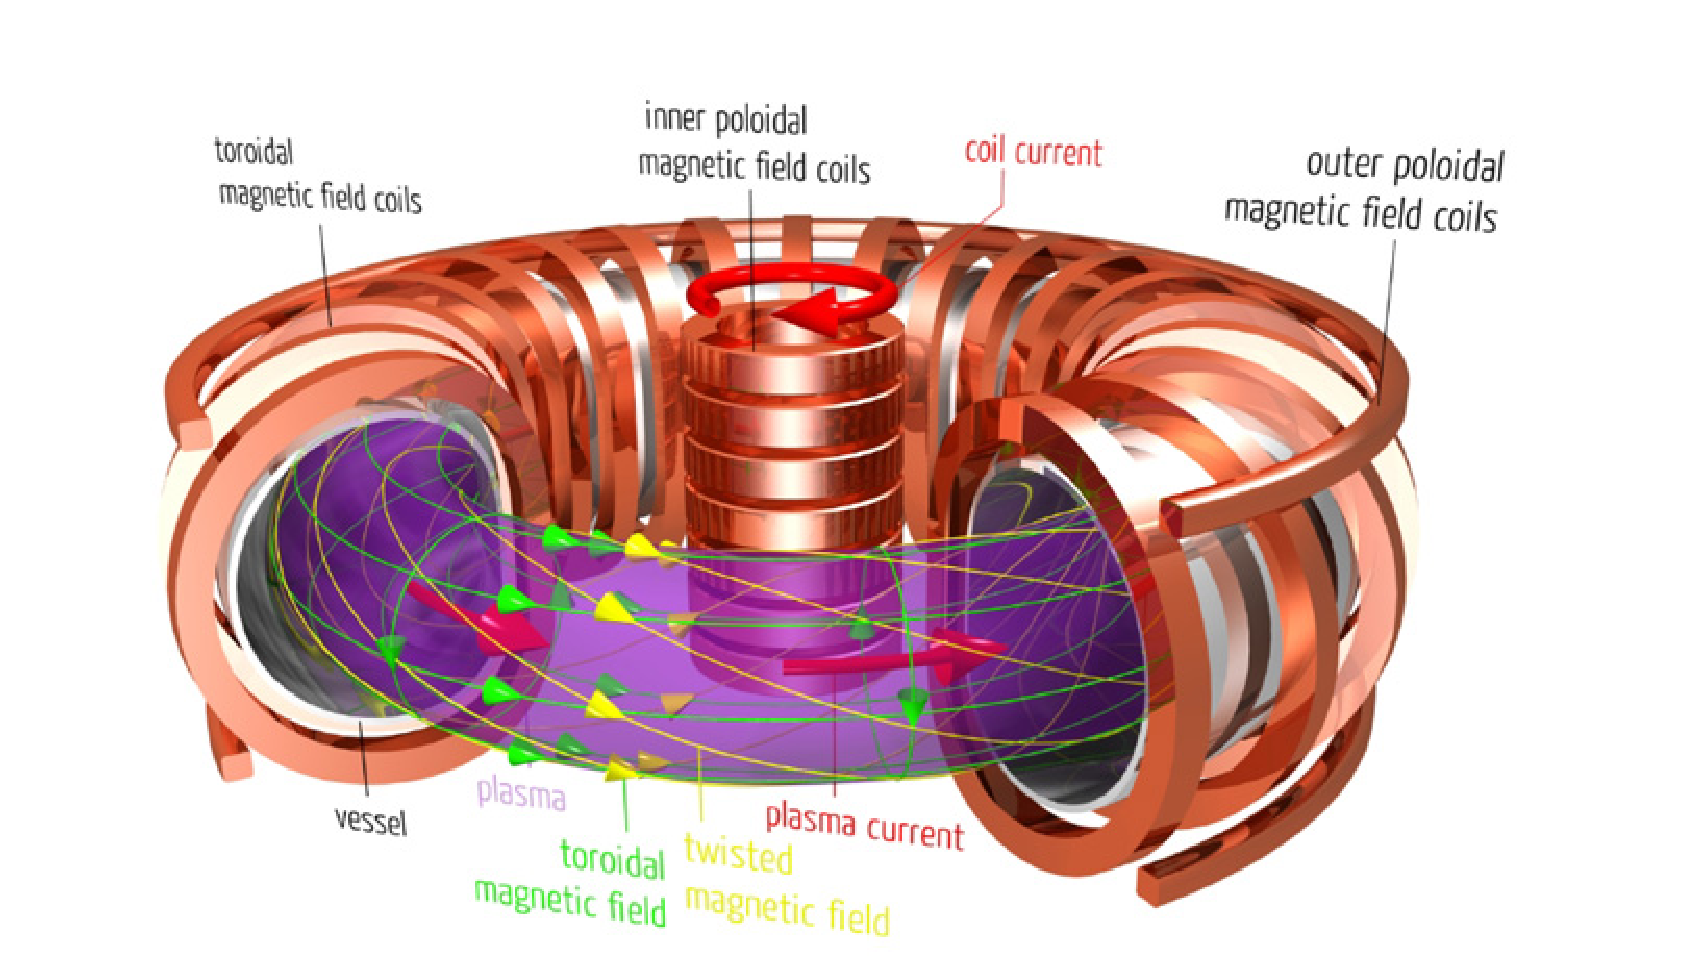
\includegraphics[width=0.9\linewidth]{Chapter5/chapter5/Fig1_Tokamak}
	\caption[Schematic of a tokamak]{Schematic of a tokamak. \\\tiny{Photo credit: Abteilung \"{O}ffentlichkeitsarbeit - Max-Planck Institut f\"{u}r Plasmaphysik. Licensed under Creative Commons BY--SA 3.0 via Wikimedia Commons}}
	\label{fig:Tokamak}
\end{figure}

\subsection{Aditya Tokamak Fusion Reactor}
\begin{table}[h]
	\centering
	\caption{Parameters of Aditya Tokamak under different power supplies}
	\label{tab:Aditya_Param}
	%	\resizebox{0.85\textwidth}{!}{%
	\begin{tabular}{cll}
		\hline
		\multicolumn{1}{l}{Power Supply} & Parameters & Approx. Values \\ \hline
		\multirow{4}{*}{Capacitor Bank} & Plasma Current & 30 kA \\
		& Shot Duration & 25 ms \\
		& Central Electron Temp. & 100 eV \\
		& Core Plasma Density & $10^{19} m^{-3}$ \\ \hline
		\multirow{4}{*}{\begin{tabular}[c]{@{}c@{}}Aditya Pulse Power\\ Supply (APPS)\end{tabular}} & Plasma Current & 100 kA \\
		& Shot Duration & 25 ms \\
		& Central Electron Temp & 100 eV \\
		& Core Plasma Density & $3 x 10^{19} m^{-3}$ \\ \hline
	\end{tabular}
	%	}
\end{table}
Aditya Tokamak Fusion Reactor (Aditya) is India's first Tokamak Fusion Test Reactor (TFTR) \cite{bhatt1989aditya}. It is a medium sized test reactor designed, developed and stationed at Institute of Plasma Research, Gandhinagar, India. The plasma has a major and minor radius of 0.75 m and 0.25 m respectively. There are twenty toroidal magnetic field coils symmetrically arranged across the torus. These coils produce a maximum magnetic field strength of 1.2 tesla. Table \ref{tab:Aditya_Param} describes the parameters of Aditya Tokamak under different power supplies.
\begin{figure}[h!]
\centering

\includegraphics[width=0.95\linewidth]{Chapter5/chapter5/Fig3_PlasmaDisplacement}
\caption[Plasma Displacement inside Vacuum Chamber]{Cross-sectional view of plasma position and displacement inside the vacuum chamber}
\label{fig:Fig5_3}
\end{figure}


\section{Aditya Tokamak System Modeling}
In this section, the control problem of radial position of plasma in Aditya TFTR using fast feedback (FF) coil has been analysed using a RZIP model. The geometric center of vacuum vessel of Aditya TFTR is at 0.75 m and it is critical that the radial position of the plasma maintained at this point. This model is developed with the assumption that small variation in coil currents produces small change in plasma position and current.  

Unlike circular cross-section plasmas, Tokamak operates on highly non-circular torus shape. Non-circular shapes are more difficult to produce and to control accurately, since currents through several control coils must be adjusted simultaneously\cite{Bishop1995}. Due to uncertainties in the current and pressure distributions within the plasma, the desired accuracy for plasma control can only be achieved by making real-time measurements of the position and shape of the boundary, and using error feedback to adjust the currents in the control coils. The modeling of the discharge parameters like plasma current, position and shape is a challenging task, as they are highly nonlinear and time varying in nature. Hence, due to inherent complexity of the plasma position control system and its nonlinear nature, it is difficult to achieve control of plasma position using traditional controllers \cite{Suratia2012}. A similar approach was also taken by Morelli et. al. \cite{Morelli2005b} in plasma position control of STOR-M Tokamak Fusion Test Reactor.

Considering the above modeling parameters taken from the work by Bandyopadhyay et. al. \cite{Bandyopadhyay2001,bandyopadhyaya2006},

\begin{equation}
\dot{X}={\bf A}X + {\bf B}U
\end{equation}

where ${\bf A}={\overline{\cal{M}}}^{-1}\cdot{\overline{\cal{R}}}$, 
${\bf B}={\overline{\cal{M}}}^{-1}$,  and
\[X = \left[ {\begin{array}{*{20}{c}}
	{{I_C}}\\
	{z{I_P}}\\
	{R{I_P}}\\
	{{I_P}}
	\end{array}} \right],U = \left[ {\begin{array}{*{20}{c}}
	{{V_C}}\\
	0\\
	{ - \frac{{{\mu _0}{I_P}}}{2}\Gamma }\\
	{{I_P}}
	\end{array}} \right]\]
$ \overline{\cal{M}} $ and $ \overline{\cal{R}} $ refers to vector of mutual inductances and resistances of all circuits with plasma \cite{bandyopadhyaya2004,bandyopadhyaya2006,Suratia2012}. 

$\overline{\cal{M}} = \left[ {\begin{array}{*{20}{c}}
	{{M_C}}&{{{\left( {M{'_R}} \right)}^T}}&{{M_{PC}}}\\
	{M{'_Z}}&0&0\\
	\begin{array}{l}
	M{'_R}\\
	{M_{PC}}
	\end{array}&\begin{array}{l}
	{M_{22}}\\
	{M_{22}}
	\end{array}&\begin{array}{l}
	{M_{22}}\\
	{L_{P0}}
	\end{array}
	\end{array}} \right]$ and $\overline{\cal{R}} = \left[ \begin{array}{l}
\begin{array}{*{20}{c}}
{{\Omega _C}}&0&0\\
0&0&0\\
0&0&0
\end{array}\\
\begin{array}{*{20}{c}}
0&{\Omega {'_P}}&{{\Omega _P}}
\end{array}
\end{array} \right]$

where, 
$\begin{array}{l}
{M_{22}} = \left( {\frac{{{\mu _0}}}{2}\frac{{d\Gamma }}{{dr}} + \frac{{2\pi {B_{z0}}}}{{{I_{p0}}}} + \frac{{2\pi {R_0}B{'_{z0}}}}{{{I_{p0}}}}} \right)\\
{M_{23}} = \left( {{\mu _0}{\Gamma _0} + \frac{{2\pi {R_0}{B_{z0}}}}{{{I_{p0}}}}} \right)\\
{M_{32}} = \left( {{\mu _0}\left( {1 + {f_0}} \right) + \frac{{2\pi {R_0}{B_{z0}}}}{{{I_{p0}}}}} \right)
\end{array}$,
${M_C}$ and ${\Omega _C}$ are mutual inductance and resistance matrices of all the circuits,
${M_{PC}}$ and ${M_R}$ are the vector of mutual inductances of the circuits with the plasma and their radial derivatives respectively, and
$\Gamma $ is known as Shafranov parameter. 
This shows that $ A $ and $ B $ are matrices of dependent on the mutual inductances and resistances of all circuits with plasma which is highly non-linear in nature. 

In Aditya TFTR, four magnetic probes are used to measure the radial position of the plasma. These probes are places close to the outer periphery of the vacuum vessel. A Rogowski coil is used to measure the plasma current ($I_P$).
\par
P. Suratia et. al. \cite{Suratia2012} and I. Bandyopadhyay et. al. \cite{bandyopadhyaya2004} explained the major control operatives as - "ADITYA has been provided with a primary vertical coil field with adjustable gain proportional to plasma current, to compensate the change in vertical displacement of plasma column. The shift in radial position due to minor disruptions is controlled by a separate pair of Fast Feedback coils, this fast feedback coils produces adequate magnetic field to bring the plasma column back to its geometrical center."

\section{Control Strategy}
\subsection{Using PID Control}
\begin{figure}[b!] 
	\centering
	
\includegraphics[width=0.95\linewidth]{Chapter5/chapter5/Fig2_ControlStrategy}
	\caption[Control Strategy for Aditya TFTR]{Control strategy for radial plasma position control in Aditya TFTR}
	\label{fig:Fig5_2}
\end{figure} 
Traditional PID controllers are used presently in Aditya TFTR to which radial position signal is fed as input. The controller generates a suitable control signal to actuate the current in the fast feedback coils and accordingly the plasma is confined in radial direction \cite{Suratia2012}. Figure \ref{fig:Fig5_2} shows the control strategy employed in radial position control of plasma in Aditya TFTR. 
\[\frac{{\Delta {B_v}}}{{{B_v}}} = \frac{{\Delta R}}{R}\]
The vertical field required to maintain the radial position of plasma in Aditya TFTR can be obtained from Grad-Shafranov equation \cite{Mukhovatov1971,Suratia2012} presented at \eqref{eq:grad}. 
\begin{equation} \label{eq:grad}
{B_v} = \frac{{{\mu _0}{I_P}}}{{4\pi R}}\left[ {\ln \left( {\frac{{8R}}{a}} \right) + {\beta _P} + \frac{{{l_i} - 3}}{2}} \right]
\end{equation}
where, 	\textbf{B} is Magnetic flux density,
$ B_\phi, B_\theta, B_\rho $ is Toroidal, poloidal and radial components of the magnetic field, $E$ is Electric field intensity, $ J $ is Plasma current density, $ R $ is Major radial coordinate and $ a $ is Minor radial coordinate.
It can be observed from \eqref{eq:grad} that, the total vertical magnetic field for proper position control of plasma is proportional to the magnitude of 
\begin{enumerate}
	\item Internal inductance of plasma $ {l_i} $,
	\item Plasma current $ I_P $, and
	\item Plasma poloidal beta\footnote{ It is the ratio of the poloidal plasma pressure to the poloidal magnetic pressure}.
\end{enumerate} 
All these parameters are time varying and highly nonlinear in nature. The limitations of PID controllers have been already explained and therefore, a controller equipped to handle these parameters to provide a smooth, fast and robust control action is of utmost importance. However, it is important to exercise the existing knowledge gathered from the system response with PID controller. A PID control loop for radial plasma position control of Aditya TFTR is developed in Simulink as shown in Figure \ref{fig:Fig5_4}. It represent the mathematical model explained in \eqref{eq:grad}. The PID controller is tuned using Ziegler\hyp{}Nichols method. The Ziegler\hyp{}Nichols tuning method is a heuristic method of tuning a PID controller \cite{bandyopadhyaya2004,bandyopadhyaya2006}. The simulation output data is observed and recorded. 
\begin{figure}[h!]
\centering
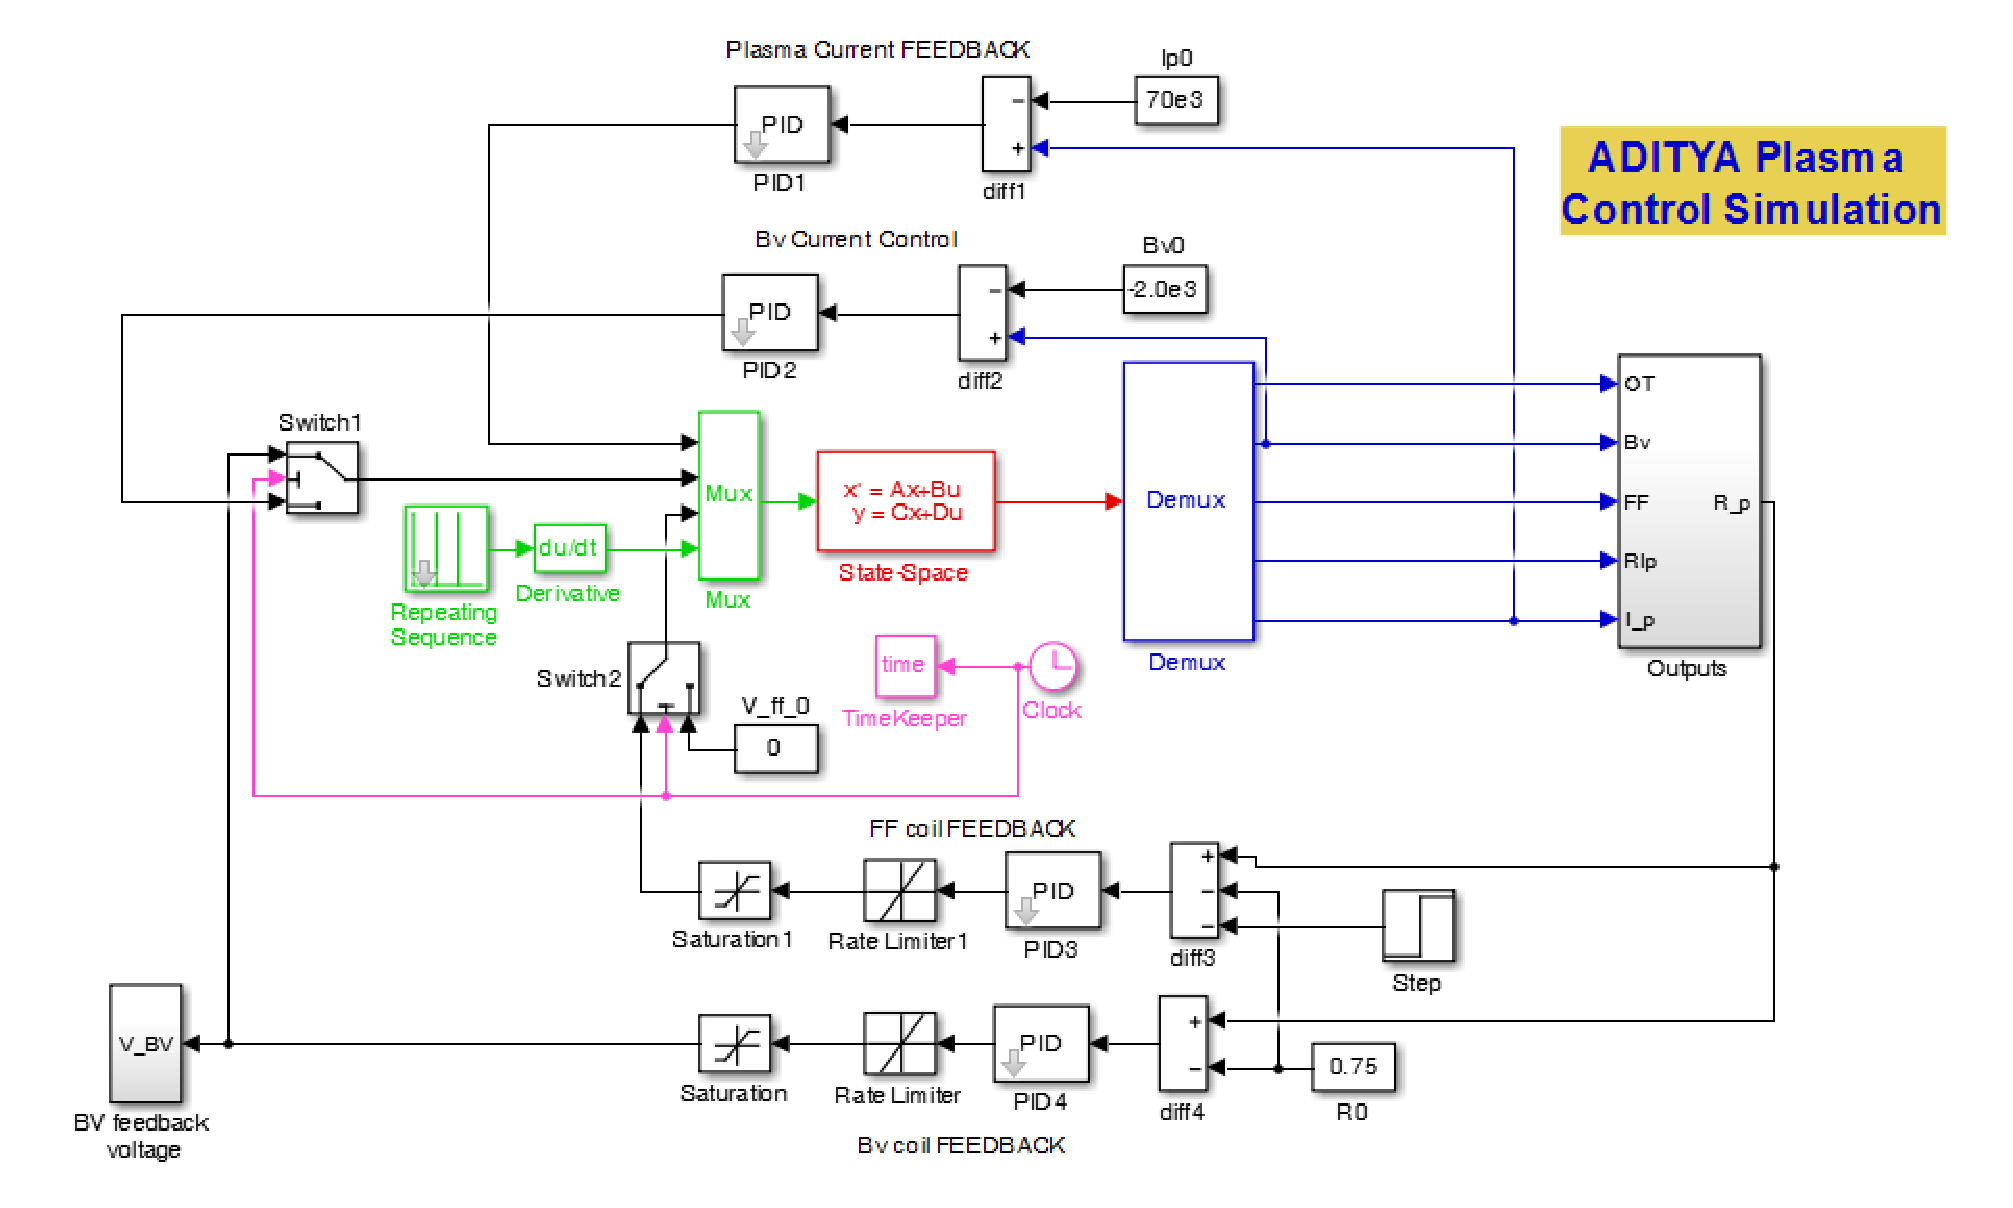
\includegraphics[width=1\linewidth]{Chapter5/chapter5/Fig5_AdityaSimPID}
\caption{Simulink model of radial plasma position control in Aditya TFTR with PID controller}
\label{fig:Fig5_4}
\end{figure}

\subsection{Plasma Position Control in Aditya using Traditional Fuzzy Logic Controller}
P. Suratia et. al. proposed a fuzzy logic controller for radial plasma position control in Aditya TFTR \cite{Suratia2012}. The characteristic features of this controller and the proposed G-FLCS used in the control simulation is tabulated in Table \ref{tab:FLC_Param}. The Simulink model with the FLC is shown in Figure \ref{fig:Fig5_5}. It can be observed in this figure that the inner PID loop in the outer position control loop in Figure \ref{fig:Fig5_4} is replaced by a FLC loop in Figure \ref{fig:Fig5_5}. The download link to the FCP used in \cite{Suratia2012} to control the radial position of plasma in Aditya TFTR is provided in Appendix-A. 
\begin{table}
	\centering
	\caption{Characteristics of FLCs used in \cite{Suratia2012} and G-FLCS}
	\label{tab:FLC_Param}
	\begin{tabular}{ccc}
		\hline Parameters & \cite{Suratia2012} & G-FLCS \\ 
		\hline Inputs & 2 & 2 \\ 
		Output & 1 & 1 \\ 
		Antecedant MFs & 7 (triangular) & 7 (trapezoidal, triangular) \\ 
		Consequent MFs & 7 (singleton) & 7 (trapezoidal, triangular) \\ 
		Aggregation & MIN & MIN \\ 
		Implication & MAX & MAX \\ 
		MF Overlapping Degree & 2 & Dynamic (4) \\ 
		Defuzzification Method & Weighted Average & CoA \\ 
		\hline 
	\end{tabular} 
\end{table}
\begin{figure}[h!]
	\centering
	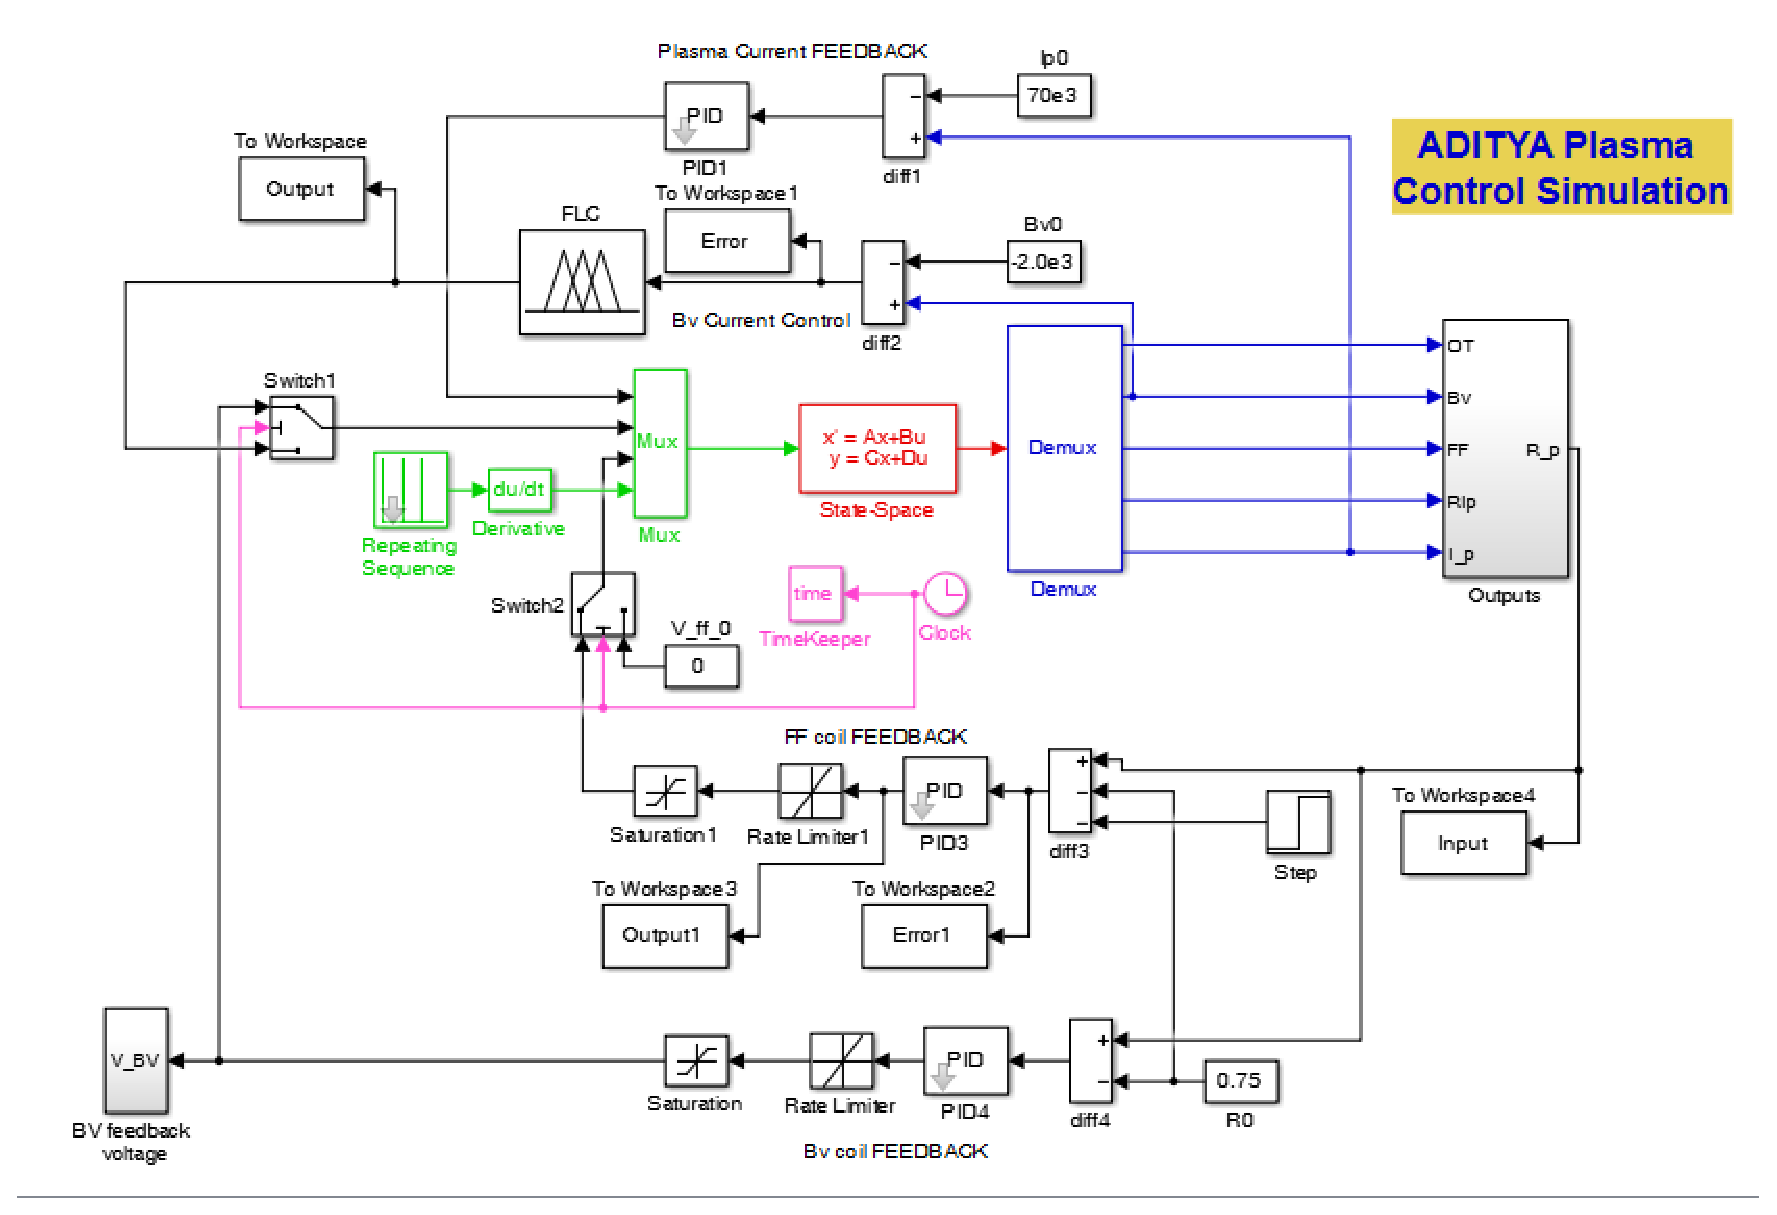
\includegraphics[width=1\linewidth]{Chapter5/chapter5/Fig4_AdityaSimFLC}
	\caption{Simulink model of radial plasma position control in Aditya TFTR with FLC}
	\label{fig:Fig5_5}
\end{figure}


\section{Introduction to Multi Objective Genetic Algorithm}
Majority of real world processes and plants operate at their best when an optimum state is achieved by balancing multiple objectives. A multi objective optimization problem is mathematically represented as \cite{OReilly2012,Whitley1994};
\[\begin{array}{l} \label{eq.5_moga}
F\left( x \right) = {\left( {{f_1}(x), \ldots ,{f_m}(x)} \right)^T}\\
x \in \Omega \nonumber
\end{array}\]
where x is a decision vector in a $ \Omega $ vector space. $ F\left( x \right) $ constitutes of $ m $ number of objective functions \[{f_i}:\Omega  \to R,\forall i \to \left[ {1,m} \right]\] 
where $ R^m $ represents the objective space. Now in \eqref{eq.5_moga}, the objective function $ f_i $, mostly experiences trade off between each other. Thus to achieve an optimal solution is important for any engineer. The best trade off solution that can be achieved using these objective functions is called the Pareto Optimal Solutions. 
\begin{Definition}\label{def:5_1} 
	An optimal feasible solution $ {x^*} \in \Omega $ in \eqref{eq.5_moga} is called a pareto optimal solution \[\text{iff }\not \exists y \in \Omega \] such that $ F\left( y \right) < F\left( {{x^*}} \right) $. Set of all pareto optimal solutions
	\[SPOS = \left\{ {x \in \Omega |\not \exists y \in \Omega ,F\left( y \right) < F\left( {{x^*}} \right)} \right\}\]	
\end{Definition} 

\begin{figure}[h!]
	\centering
	
\includegraphics[width=0.9\linewidth]{Chapter5/chapter5/Fig12_GA_Flow}
	\caption{Flowchart of Genetic Algorithm}
	\label{fig:Fig12_GA_Flow}
\end{figure}
Evolutionary algorithms like GA, PSO and others where population based heuristic search is conducted, can successfully approximate the whole $ SPOS $ of a multi objective optimization problem. Genetic Algorithm (GA) is arguably most widely used search heuristic in the field of artificial intelligence and machine learning. It is inspired by Darwin's theory of evaluation and natural selection \cite{Whitley1994}. Figure \ref{fig:Fig12_GA_Flow} provides a general block diagram to the basic outline as follows.
\begin{description}
	\item[Initial Population] To generate $ P_0 $ set of valid parameters in accordance to the parameter constraints. This individual set of parameters are called chromosomes.
	\item[Fitness] To evaluate fitness $ F(x) $ for each chromosome $ x $ in the population $ P_0 $ and $ P_k = P_0 $.
	\item[Stopping Condition Check] Check if the stopping conditions for all objectives are met. If \textit{yes} then exit and return parameter set with best fitness value.
	\item[New Population] New population can be selected from existing $P_k$ following the steps mentioned below.
	\begin{description}
		\item[a. Selection] Select $n$ best fitness chromosome from $ P_k $. These represents the [arent chromosomes. Reject others.]
		\item[b. Crossover] With the probability for crossover, generate new offspring.
		\item[c. Mutation] With mutation probability, mutate the new offspring.
		\item[d. Acceptance] Generate the population $ P_k $ using new population.
	\end{description}
	\item[Loop] Go to Fitness.
\end{description}  

\section{GA based FCP Extraction}
In this section, a GSA based FCP extraction for Aditya TFTR is presented. The details of the parameters to be tuned using GS are presented in section \ref{sec:ident_param}. The optimization problem is as follows.
Tune sixty-one FCP as mentioned in \ref{sec:ident_param} such that the response of the TFTR fulfils the objectives of
\begin{enumerate}
	\item settling time,
	\item transient time, and
	\item steady state error.
\end{enumerate}

All these corresponds to as minimum optimization problem. 

\begin{figure}[h!]
	\centering
	
\includegraphics[width=1\linewidth]{Chapter5/chapter5/Fig12_GA_Full_Flowchart}
	\caption{Flowchart of Genetic Algorithm}
	\label{fig:Fig12_GA_Full_Flowchart}
\end{figure}
Genetic algorithm based fuzzy parameter extraction scheme, as explained in section \ref{sec:FCP}, is implemented to derive the FCP to control radial position of plasma in Aditya TFTR model as shown in Figure \ref{fig:Fig5_5}. The extracted FCP is provided in Appendix B. 
\subsection{FLC I/O Identification}
The parameters that is considered are \\
$R_P$ Error~~~~~$\rightarrow$ Input with 7 MFs (Triangular and Trapezoidal) \\
$I_P$~~~~~~~~~~~$\rightarrow$ Input with 7 MFs (Triangular and Trapezoidal) \\
Control Signal~~$\rightarrow$ Output with 7 MFs (Triangular and Trapezoidal)

\subsection{FLC Parameter Identification} \label{sec:ident_param}
$ \left( i\right)  $ Radial Position Error $R_P$:\\
Range $\rightarrow$ $ \left[ -0.05, 0.05\right] $ \\
Parameters:
\[\left[ \begin{array}{l}
\left( {{R_{{P_{1A}}}},{R_{{P_{1B}}}}} \right),\left( {{R_{{P_{2A}}}},{R_{{P_{2B}}}},{R_{{P_{2C}}}}} \right),\left( {{R_{{P_{3A}}}},{R_{{P_{3B}}}},{R_{{P_{3C}}}}} \right),\left( {{R_{{P_{4A}}}},{R_{{P_{4B}}}},{R_{{P_{4C}}}}} \right),\\
\left( {{R_{{P_{5A}}}},{R_{{P_{5B}}}},{R_{{P_{5C}}}}} \right),\left( {{R_{{P_{6A}}}},{R_{{P_{6B}}}},{R_{{P_{6C}}}}} \right),\left( {{R_{{P_{7A}}}},{R_{{P_{7B}}}}} \right)
\end{array} \right]\]
Number of parameters $n_{R_P} = 19$
\begin{figure}[h!]
\centering

\includegraphics[width=0.95\linewidth]{Chapter5/chapter5/Fig7_FCP_Rp}
\caption{MF co-ordinates for Parameter Extraction: Radial Position Error}
\label{fig:Fig5_7}
\end{figure}

\par
\noindent$ \left( ii\right) $ Plasma Current $I_P$: \\
Range $\rightarrow$ $ \left[ 5e4, 8e4\right] $ \\
Parameters:
\[\left[ \begin{array}{l}
\left( {{I_{{P_{1A}}}},{I_{{P_{1B}}}},{I_{{P_{1C}}}}} \right),\left( {{I_{{P_{2A}}}},{I_{{P_{2B}}}},{I_{{P_{2C}}}}} \right),\left( {{I_{{P_{3A}}}},{I_{{P_{3B}}}},{I_{{P_{3C}}}}} \right),\left( {{I_{{P_{4A}}}},{I_{{P_{4B}}}},{I_{{P_{4C}}}}} \right),\\
\left( {{I_{{P_{5A}}}},{I_{{P_{5B}}}},{I_{{P_{5C}}}}} \right),\left( {{I_{{P_{6A}}}},{I_{{P_{6B}}}},{I_{{P_{6C}}}}} \right),\left( {{I_{{P_{7A}}}},{I_{{P_{7B}}}},{I_{{P_{7C}}}}} \right)
\end{array} \right]\]
Number of parameters $n_{I_P} = 21$
\begin{figure}[h!]
	\centering
	
\includegraphics[width=0.95\linewidth]{Chapter5/chapter5/Fig8_FCP_Ip}
	\caption{MF co-ordinates for Parameter Extraction: Plasma Current}
	\label{fig:Fig5_8}
\end{figure}

\par
\noindent$ \left( iii\right) $ Control Signal $u$: \\
Range $\rightarrow$ $ \left[ -60, 60\right] $ \\
Parameters:
\[\left[ \begin{array}{l}
\left( {{u_{1A}},{u_{1B}},{u_{1C}}} \right),\left( {{u_{2A}},{u_{2B}},{u_{2C}}} \right),\left( {{u_{3A}},{u_{3B}},{u_{3C}}} \right),\left( {{u_{4A}},{u_{4B}},{u_{4C}}} \right),\\
\left( {{u_{5A}},{u_{5B}},{u_{5C}}} \right),\left( {{u_{6A}},{u_{6B}},{u_{6C}}} \right),\left( {{u_{7A}},{u_{7B}},{u_{7C}}} \right)
\end{array} \right]\]
Number of parameters $n_{I_P} = 21$
\begin{figure}[h!]
	\centering
	
\includegraphics[width=0.95\linewidth]{Chapter5/chapter5/Fig9_FCP_u}
	\caption{MF co-ordinates for Parameter Extraction: Control Signal}
	\label{fig:Fig5_9}
\end{figure}

\subsection{Parameter Constraints}
There are total of sixty one identified parameters in section \ref{sec:ident_param}. The shape of the membership functions are dependent of these parameters and therefore the relationship between these parameters are cardinal. Genetic algorithm is well equipped to handle these nonlinear equality constraints between the parameters. Listing \ref{CS:constraints}
%\lstset{,caption={},label={}}
\begin{lstlisting}[language=Matlab,caption={Describing nonlinear equality constraints},label=CS:constraints]
function [c, ceq] = confun_FLC(X)

% Nonlinear equality constraints
c = [X(1) + 0.001 - X(2);       % Input Rp Starts Here
X(3) + 0.001 - X(4);      X(4) + 0.001 - X(5);
X(6) + 0.001 - X(7);      X(7) + 0.001 - X(8);
X(9) + 0.001 - X(10);     X(10) + 0.001 - X(11);
X(12) + 0.001 - X(13);    X(13) + 0.001 - X(14);
X(15) + 0.001 - X(16);    X(16) + 0.001 - X(17);
X(18) + 0.001 - X(19);      % Input Rp Ends Here
X(20) + 5 - X(21);      % Control Output u starts here
X(21) + 5 - X(22);    X(23) + 5 - X(24);
X(24) + 5 - X(25);    X(26) + 5 - X(27);
X(27) + 5 - X(28);    X(29) + 5 - X(30);
X(30) + 5 - X(31);    X(32) + 5 - X(33);
X(33) + 5 - X(34);    X(35) + 5 - X(36);
X(36) + 5 - X(37);    X(38) + 5 - X(39);
X(39) + 5 - X(40)];     % Control Output u Ends Here

% Nonlinear equality constraints

ceq = [];
\end{lstlisting}

\subsection{Parameter Extraction}
\begin{figure}[h!]
\centering

\includegraphics[width=0.7\linewidth]{Chapter5/chapter5/Fig10_AdityaFCP_Extraction}
\caption[Block Diagram for FCP Extraction for $R_P$ Control]{Block Diagram for FCP Extraction for Radial Position Control in Aditya TFTR}
\label{fig:Fig5_10}
\end{figure}
In Figure \ref{fig:Fig5_10}, the parameter extraction mechanism is graphically represented. Aditya TFTR Radial Plasma Position Control Simulink model is the fitness function used in GA based FCP extraction. ``$ sim $'' command in Matlab is used to execute the Simulink model from the GA Matlab script. The operation can be seen in the Code Snippet 5.2. The \textit{Error Calculation} block in Figure \ref{fig:Fig5_10} represents the objectives computed from the cost function. These objectives are 
\begin{enumerate}
	\item settling time,
	\item transient time, and
	\item steady state error.
\end{enumerate} 

\lstset{language=Matlab,caption={Fitness Function},label=CS:Fitness}
\begin{lstlisting}
simOut = sim('aditya_fast','SimulationMode','normal','AbsTol','1e-5',...
'StopTime', '0.03', ... 
'ZeroCross','on', ...
'SaveTime','on','TimeSaveName','tout', ...
'SaveState','on','StateSaveName','xoutNew',...
'SaveOutput','on','OutputSaveName','youtNew',...
'SignalLogging','on','SignalLoggingName','logsout');
results = simOut.get( 'youtNew' );
t = simOut.get( 'tout' );
\end{lstlisting}


\lstset{language=Matlab,caption={Fitness Computation},label=CS:FitComp}
\begin{lstlisting}
%Steady State Error Calculation
errOut = ((0.75 - results(end))^2)^0.5; 

% Calculation of Settling Time and Rise Time
results = simOut.get( 'youtNew' );
t = simOut.get( 'tout' );
sTime = stepinfo(results,t,0.749721);
\end{lstlisting}

\section{FLC Design and Implementation}
The extracted parameters for the radial position control provides the default FCP for the proposed G-FLCS as discussed in the earlier chapters. The extracted FCP is described in Appendix - B. G-FLCS is connected serially through UART to the server. An optimized code for FLC with MT-FRHC ispreloaded in the SHRAM of the C6748 DSP development kit. This system is prepared for a HIL test to control the plasma position. In the Simulink model presented in Figure \ref{fig:Fig5_6}, the plasma position control is achieved using three different controller mechanisms, namely, 
\begin{itemize}
	\item Tradition PID controller tuned by Ziegler--Nichols method
	\item FLC as described by P. Suratia et. al. to control radial position of plasma in Aditya TFTR
	\item G-FLCS with GA based FCP extraction scheme
\end{itemize}
\subsection{HIL Testing}
The G-FLCS is connected to a PC with Simulink model of radial plasma position control of Aditya TFTR. Using UART, data can be exchanged between the two system. The hardware G-FLCS polls for any input at the UART. Once it receives the input, it completes the FLC with MT-FRHC execution process to return a suitable control signal to the power supply of the feedback output. This completes a HIL loop and it is continued for the entire simulation. Simulation for other controllers are carried out sequentially by chnaging the manual switches as shown in Figure \ref{fig:Fig5_6}. These simulation data are recorded for all control schemes and analyzed for the performance of the controllers.
\begin{figure}[h!]
\centering
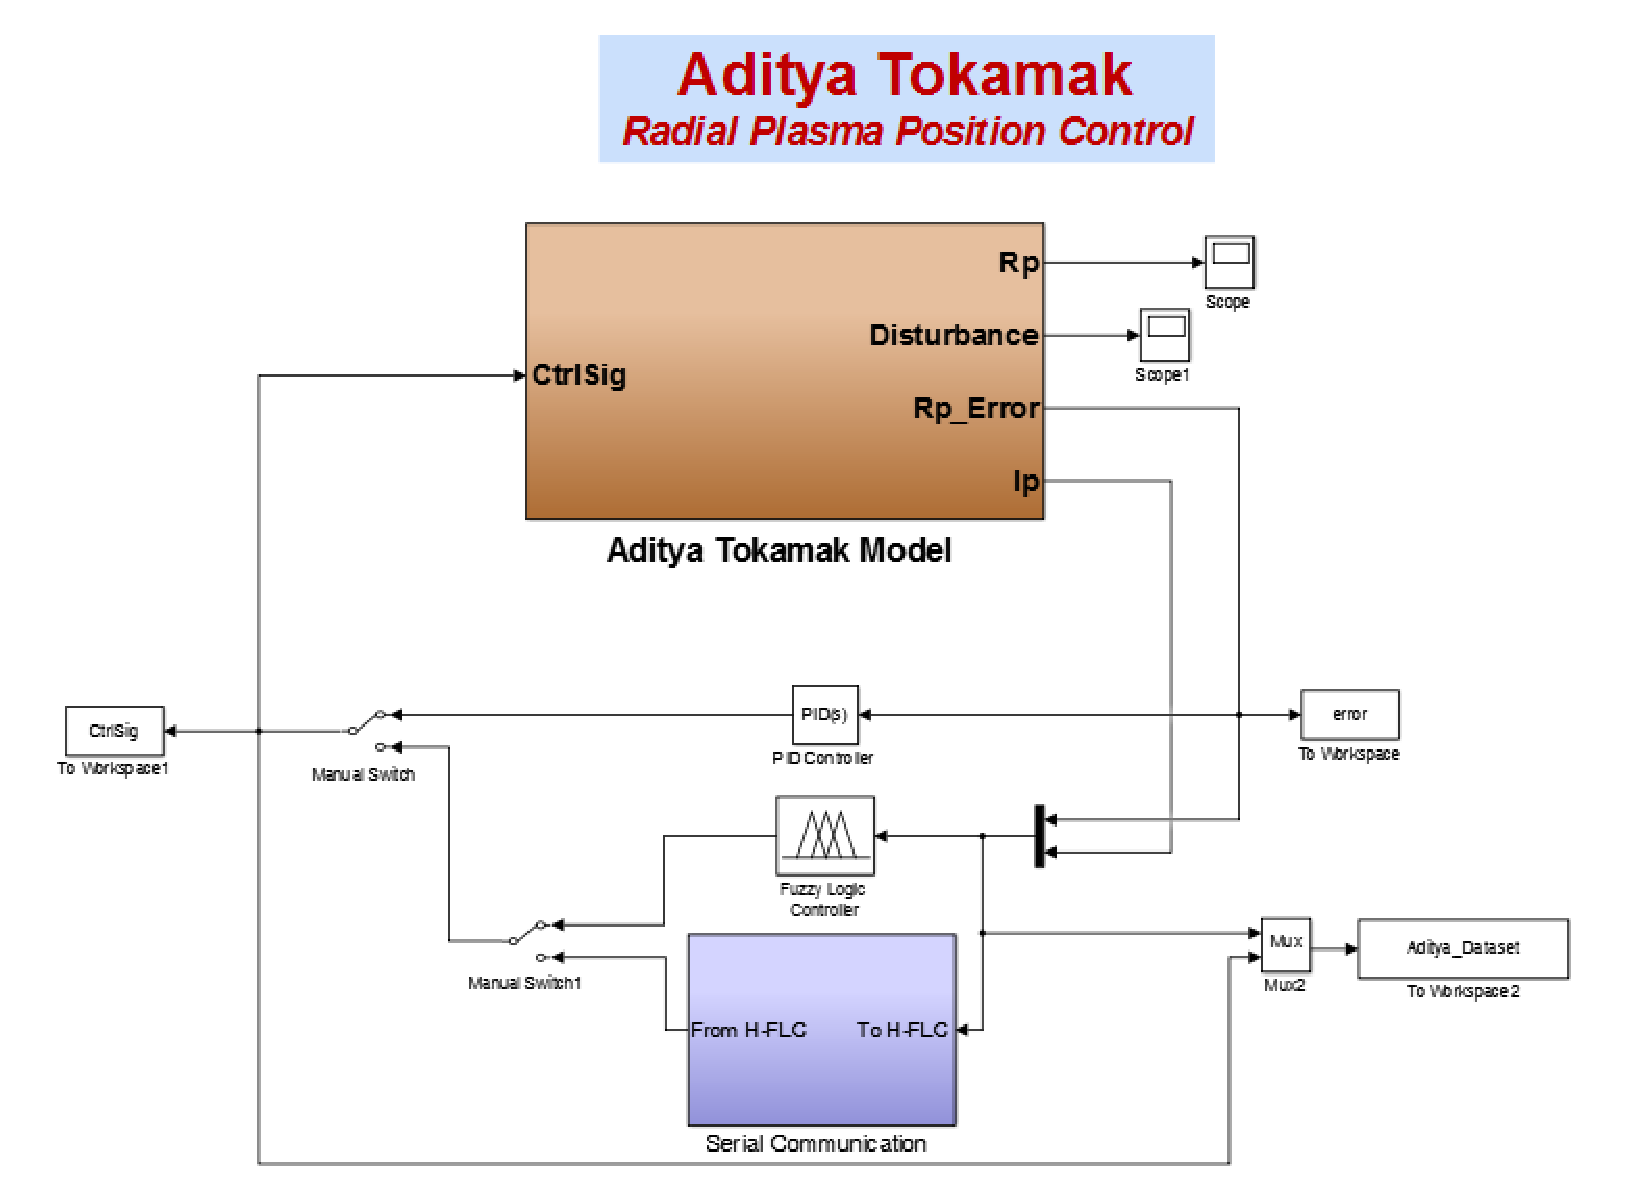
\includegraphics[width=0.95\linewidth]{Chapter5/chapter5/Fig6_AdityaSim_All}
\caption[HIL Simulation with PID, FLC\cite{Suratia2012} and G-FLCS]{Radial Plasma Position Control of Aditya TFTR: HIL Simulation with PID, FLC\cite{Suratia2012} and G-FLCS}
\label{fig:Fig5_6}
\end{figure}




\section{Performance Analysis}
The recorded data from the simulations explained in previous section is plotted as depicted in Figure \ref{fig:Fig11_Final_Figure_PhD}. This plot clearly displays the difference in the control action. A significant improvement in rise time and settling time is observed in accordance to the PID controller and existing FLC. The hardware G-FLCS is observed to provide a smooth and fast response. It caters a robust control scheme for the radial position control in Aditya TFTR. A comparative analysis of the control parameters are drawn and tabulated in Table. \ref{tab:5_comp}. It can be observed that the G-FLCS 59\% faster rise time and 87\% speedy settling time in comparison to existing control schemes. However, a slight overshoot of 0.0009 m is reported by the proposed G-FLCS. This overshoot implies a plasma displacement of 9 mm in a vacuum chamber of 750 mm which is effectively 1.2 \% of the radius.
%\begin{figure}
%\centering
%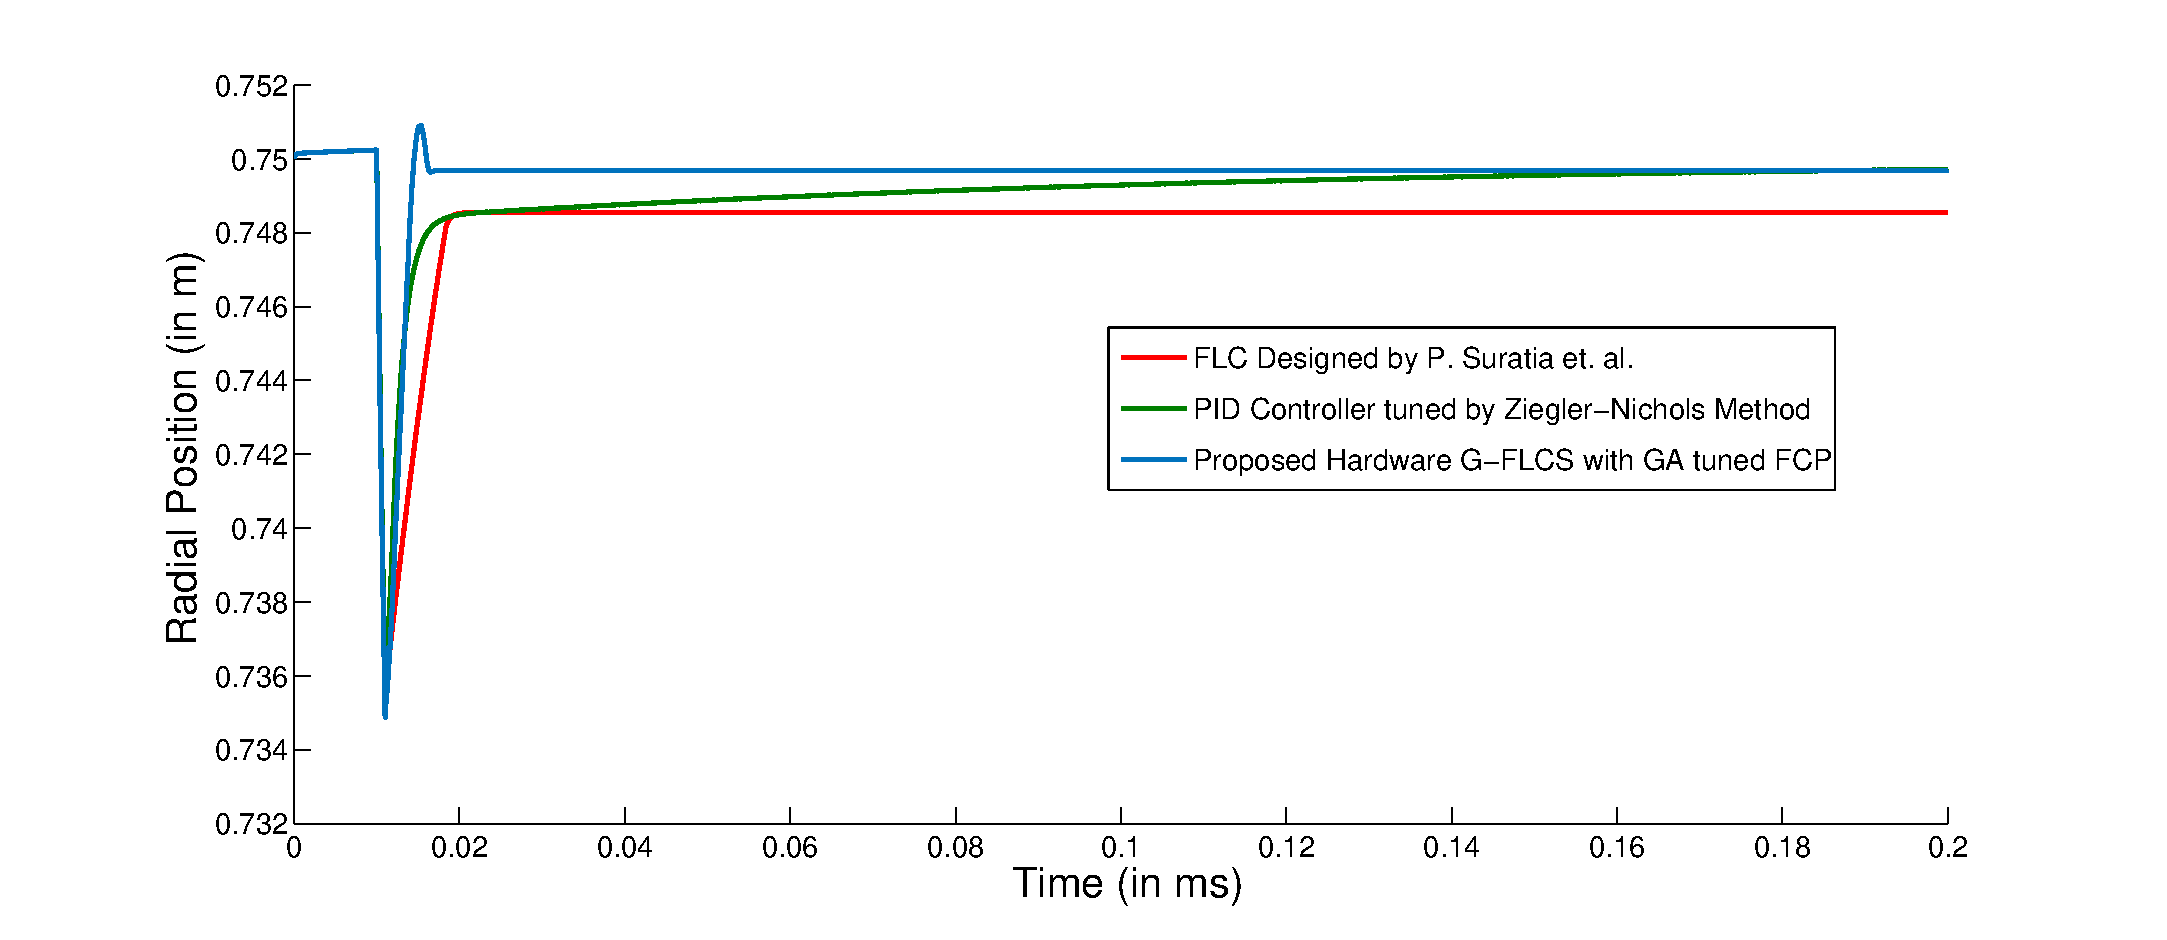
\includegraphics[width=1\linewidth]{Chapter5/chapter5/Fig11_Final_Figure_PhD}
%\caption{Performance of various controllers in presence of disturbances in plasma position}
%\label{fig:Fig11_Final_Figure_PhD}
%\end{figure}

\begin{figure}[h!]
	\centering
	\subfloat[Input Disturbance Signal]{\label{fig:Fig11_Final_Figure_PhD_in}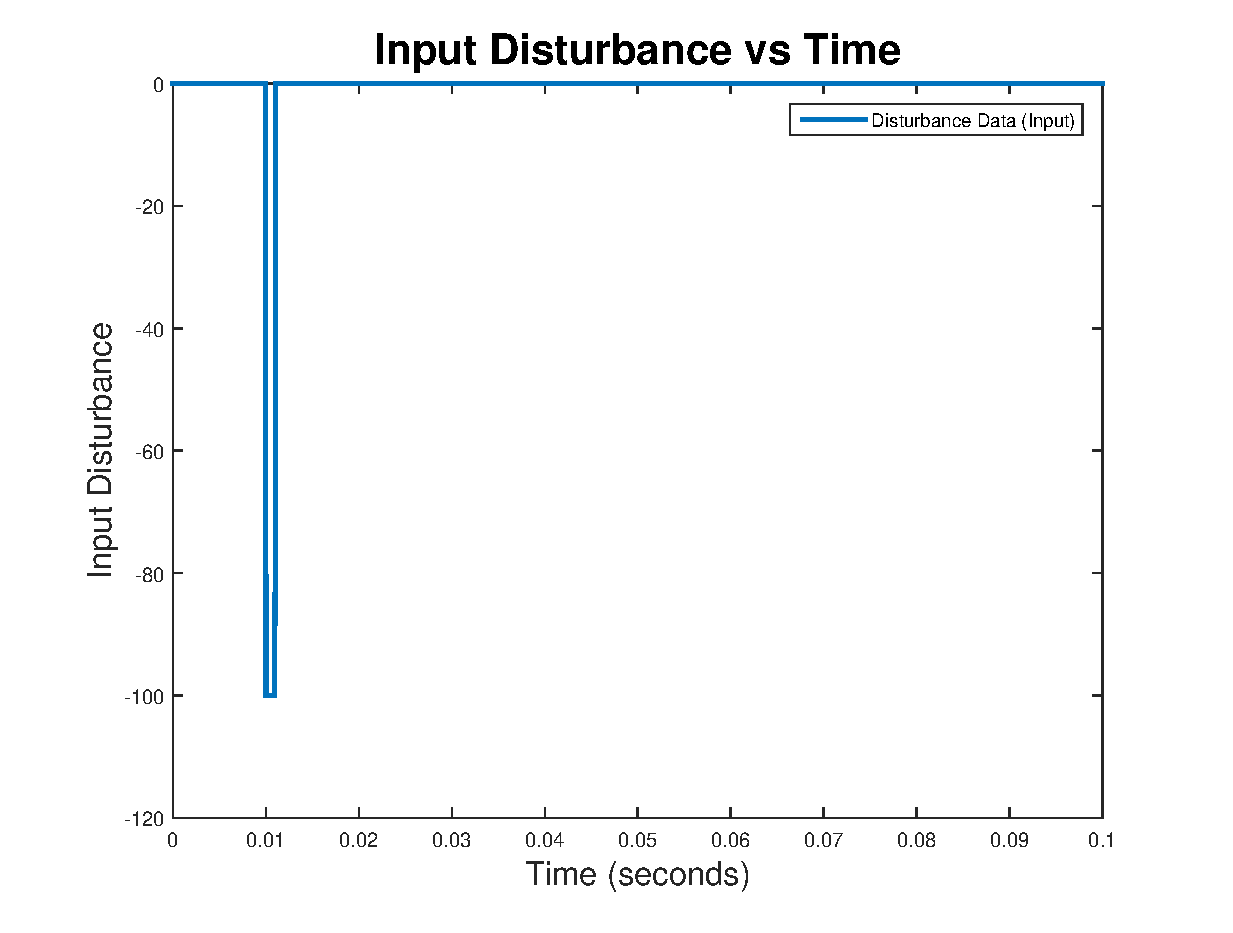
\includegraphics[width=0.95\linewidth]{Chapter5/chapter5/input_disturbance}} \\
	\subfloat[System Response]{\label{fig:Fig11_Final_Figure_PhD_op}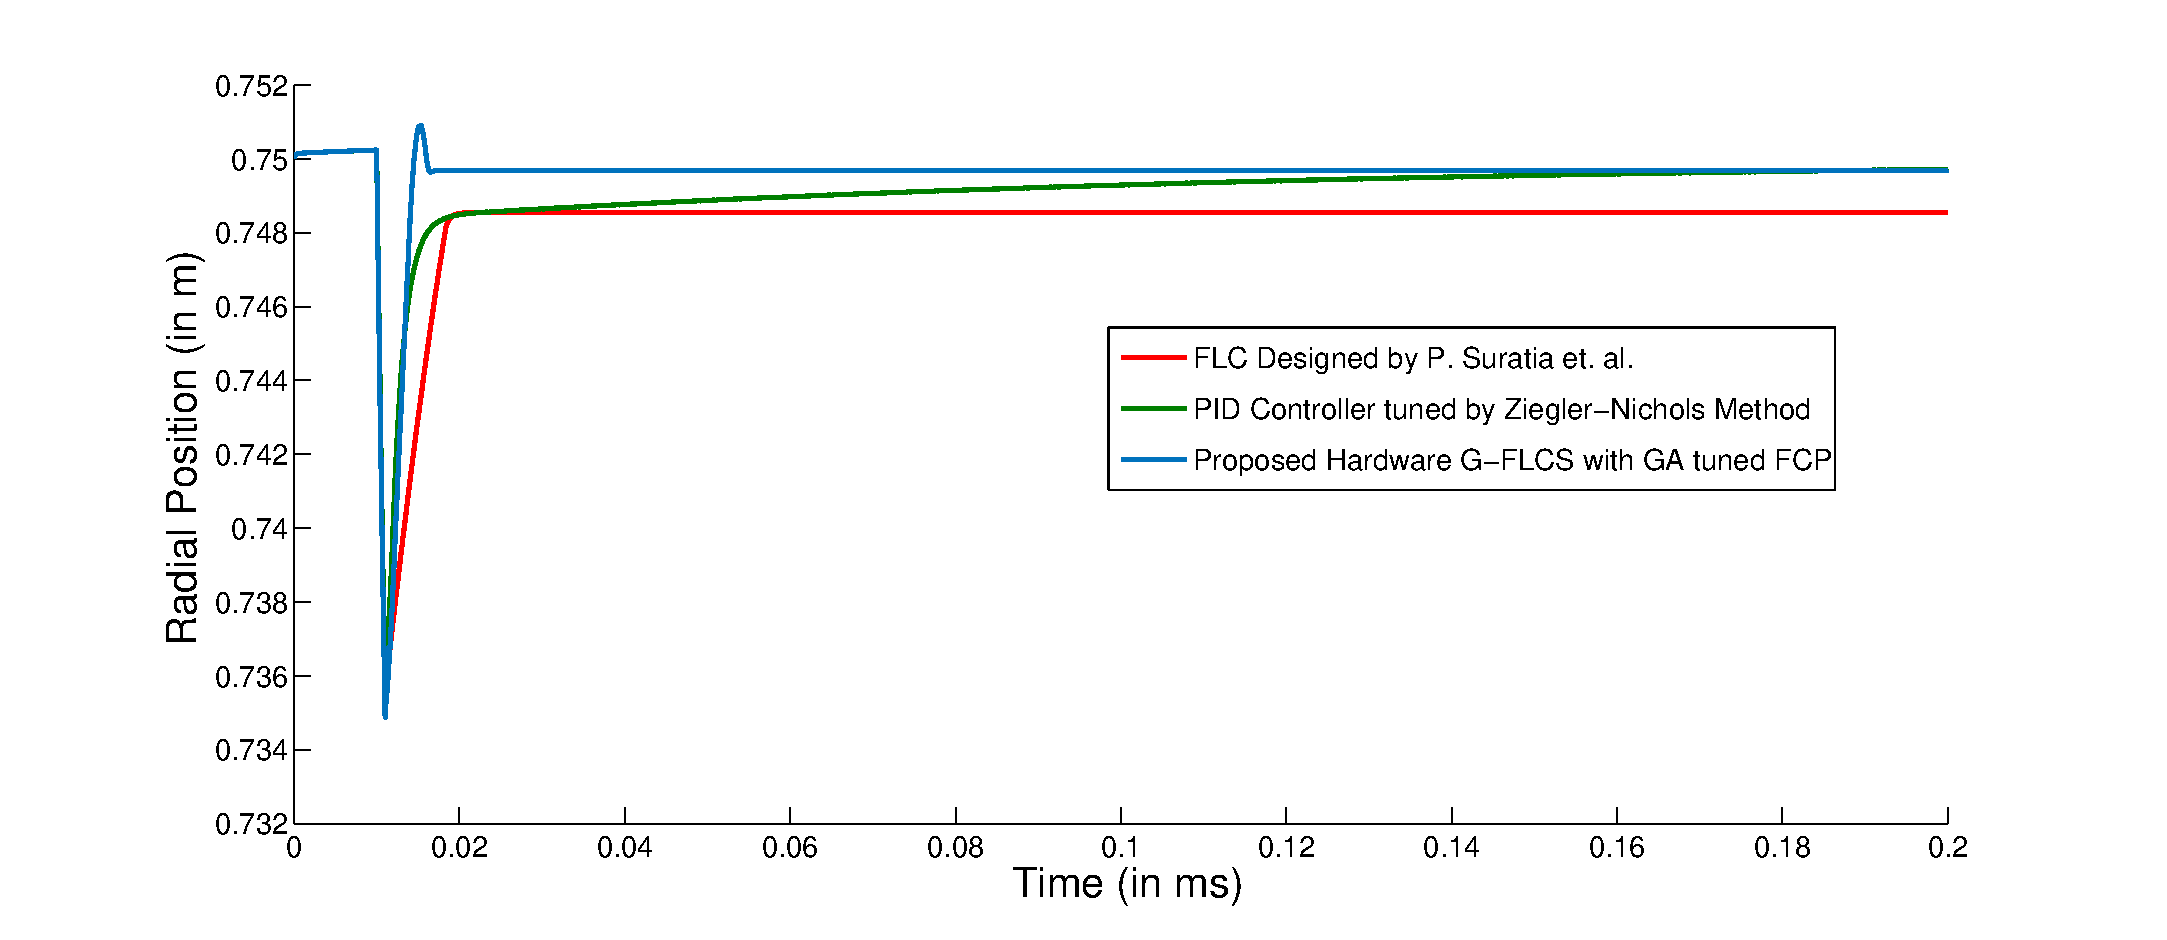
\includegraphics[width=0.95\linewidth]{Chapter5/chapter5/Fig11_Final_Figure_PhD}}
	\caption{Performance of various controllers in presence of disturbances in plasma position} 
	\label{fig:Fig11_Final_Figure_PhD}
\end{figure}

\begin{table}[h!]
	\centering
	\caption{Comparison of performance parameters of PID, FLC\cite{Suratia2012} and G-FLCS}
	\label{tab:5_comp}
	\begin{tabular}{lccc}
		\hline
		Parameters & PID & FLC\cite{Suratia2012} & GFLCS \\ \hline
		Rise Time & 0.0062 & 0.0062 & 0.0025 \\
		Settling Time & 0.1255 & NaN & 0.0160 \\
		Settling Min & 0.7483 & 0.7474 & 0.7483 \\
		Settling Max & 0.7497 & 0.7486 & 0.7509 \\
		Overshoot & 0 & 0 & 0.0009 \\
		Undershoot & 0 & 0 & 0 \\
		Peak & 0.7497 & 0.7486 & 0.7509 \\
		Peak Time & 0.2 & 0.0235 & 0.0154 \\ \hline
	\end{tabular}
\end{table}
\section{Summary}
This chapter implements the proposed MT-FRHC based G-FLCS with VBCoA on C6748 DSP in a critical and highly nonlinear control problem. In Aditya TFTR, the confinement of plasma within the vacuum chamber is crucial. Therefore, this system requires a fast and robust control algorithm. The GA based FCP extraction algorithms generates the parameters to drive the hardware G-FLCS. The proposed controller is then serially interfaced to the Simulink model through UART and tested with other control applications. The observation obtained from this system was exciting as it provided 59\% faster rise time and 87\% speedy settling time in comparison to existing control schemes. These results are extremely positive and encouraging.    
